\documentclass[aspectratio=169,10pt]{beamer}
\usepackage{fontspec}
\setmainfont{Times New Roman}[
  Path=/mnt/c/Windows/Fonts/,
  UprightFont=times.ttf,
  BoldFont=timesbd.ttf,
  ItalicFont=timesi.ttf,
  BoldItalicFont=timesbi.ttf
]
\setsansfont{Arial}[
  Path=/mnt/c/Windows/Fonts/,
  UprightFont=arial.ttf,
  BoldFont=arialbd.ttf,
  ItalicFont=ariali.ttf,
  BoldItalicFont=arialbi.ttf
]
\usepackage{graphicx}
\graphicspath{{../figures/}}
\usepackage{booktabs,tabularx,array}
\usepackage{tikz}
\usepackage{amsmath}
\usepackage{ragged2e}
\usepackage{hyperref}

\definecolor{tietmaroon}{HTML}{7A1F2B}
\definecolor{ink}{HTML}{20262E}
\definecolor{muted}{HTML}{5E6872}
\definecolor{paper}{HTML}{FAF9F6}
\definecolor{rulegray}{HTML}{D7DADF}
\definecolor{softmaroon}{HTML}{E9D8DB}
\definecolor{softgreen}{HTML}{DDE8DF}

\setbeamercolor{normal text}{fg=ink,bg=paper}
\setbeamercolor{structure}{fg=tietmaroon}
\setbeamercolor{frametitle}{fg=ink,bg=paper}
\setbeamercolor{alerted text}{fg=tietmaroon}
\setbeamerfont{frametitle}{series=\bfseries,size=\Large}
\setbeamerfont{title}{series=\bfseries,size=\Large}
\setbeamertemplate{navigation symbols}{}
\setbeamertemplate{itemize item}{\raise0.2ex\hbox{\scriptsize\color{tietmaroon}$\blacksquare$}}
\setbeamertemplate{itemize subitem}{\raise0.2ex\hbox{\tiny\color{muted}$\blacksquare$}}
\setbeamertemplate{frametitle}{%
  \vspace{0.25em}\insertframetitle\par
  \vspace{0.15em}{\color{tietmaroon}\rule{\textwidth}{0.8pt}}
}
\setbeamertemplate{footline}{%
  \leavevmode
  \hbox{%
    \begin{beamercolorbox}[wd=.82\paperwidth,ht=2.6ex,dp=1.2ex,leftskip=0.45cm]{normal text}
      \scriptsize CPG44 Football Intelligence Platform
    \end{beamercolorbox}%
    \begin{beamercolorbox}[wd=.18\paperwidth,ht=2.6ex,dp=1.2ex,rightskip=0.45cm plus1fil]{normal text}
      \scriptsize\hfill \insertframenumber/15
    \end{beamercolorbox}%
  }
}
\setbeamertemplate{headline}{}

\newcommand{\smallsource}[1]{\vfill{\tiny\color{muted}#1}}
\newcommand{\phimage}[2]{%
  \IfFileExists{../figures/#1}{\includegraphics[width=\linewidth,height=#2,keepaspectratio]{#1}}{%
  \fbox{\begin{minipage}[c][#2][c]{0.92\linewidth}\centering\bfseries Image placeholder\\[0.3em]\normalfont\scriptsize\nolinkurl{figures/#1}\end{minipage}}}%
}
\newcommand{\statusbar}[3]{%
  \begin{tikzpicture}[baseline]
    \node[anchor=west,font=\scriptsize] at (0,0.30) {#1};
    \fill[rulegray] (0,-0.11) rectangle (3.15,0.11);
    \fill[#3] (0,-0.11) rectangle ({3.15*#2/100},0.11);
    \node[anchor=west,font=\scriptsize\bfseries] at (3.28,0) {#2\%};
  \end{tikzpicture}%
}

\title{Predictive and Tactical Intelligence System for Athlete Performance}
\subtitle{Vision-Based Tracking and Wearable Data Analytics}
\author{Capstone Project Group 44}
\institute{Department of Computer Science and Engineering\\Thapar Institute of Engineering and Technology}
\date{Mid-Semester Panel Evaluation, August 22, 2026}

\begin{document}

% 1
\begin{frame}[plain]
\begin{columns}[T,onlytextwidth]
\begin{column}{0.76\textwidth}
\vspace{0.35cm}
{\color{tietmaroon}\rule{1.2cm}{2pt}}\\[0.32cm]
{\LARGE\bfseries Predictive and Tactical Intelligence System for Athlete Performance}\par
\vspace{0.16cm}
{\large Vision-Based Tracking and Wearable Data Analytics}\par
\vspace{0.4cm}
{\normalsize Siddartha Nepal \enspace Raghav Agrawal \enspace Bibek Kumar Thagunna\\
Suyogya Sedhai \enspace Om Narayan Yadav}\par
\vspace{0.25cm}
{\normalsize Project Mentor: \textbf{Dr. Saif Nalband}}\par
\vfill
{\small CPG 44 \quad Mid-Semester Panel \quad August 22, 2026}
\end{column}
\begin{column}{0.20\textwidth}
\centering

\includegraphics[width=0.95\linewidth]{tietlogo.jpg}
\end{column}
\end{columns}
\end{frame}

% 2
\begin{frame}{Problem Definition}
\begin{columns}[T,onlytextwidth]
\begin{column}{0.52\textwidth}
\textbf{Current problem}
\begin{itemize}
  \item Video explains player and ball movement.
  \item Wearables explain physical and physiological load.
  \item Separate clocks and identities make joint interpretation unreliable.
  \item A correct value assigned to the wrong player or second is still wrong.
\end{itemize}
\end{column}
\begin{column}{0.44\textwidth}
\textbf{Project response}
\begin{itemize}
  \item One calibrated live timeline
  \item Track-to-player-to-device binding
  \item Quality-aware wearable measurements
  \item Explainable tactical and load indicators
  \item Local processing with required live relay
\end{itemize}
\end{column}
\end{columns}
\vspace{0.25cm}
\begin{beamercolorbox}[rounded=false,sep=0.25cm]{block body}
\centering\bfseries Goal: evidence a coach can inspect and act upon during or after a session.
\end{beamercolorbox}
\end{frame}

% 3
\begin{frame}{Scope and Approved Objectives}
\small
\begin{enumerate}
  \item Develop an integrated system for vision-based player tracking and real-time wearable data streaming.
  \item Design and implement wearable hardware incorporating GPS, accelerometer, and pulse oximeter sensors.
  \item Develop machine-learning fusion for player and team performance, with a tactical decision-support module.
  \item Evaluate the system on public datasets and controlled scenarios using suitable accuracy measures.
\end{enumerate}
\vspace{0.25cm}
\begin{columns}[T,onlytextwidth]
\begin{column}{0.49\textwidth}
\textbf{Included now}\par
Single calibrated camera, player/ball tracking, team and jersey identity, ESP32-S3 relay stream, local dashboard, tactical and workload features.
\end{column}
\begin{column}{0.49\textwidth}
\textbf{Safety boundary}\par
Load and recovery decision support. No medical diagnosis, certified SpO$_2$ claim, or automatic referee decision.
\end{column}
\end{columns}
\end{frame}

% 4
\begin{frame}{Literature Findings and Research Gap}
\scriptsize
\begin{tabularx}{\textwidth}{p{2.5cm}X X}
\toprule
\textbf{Area} & \textbf{What prior work provides} & \textbf{Gap addressed here}\\
\midrule
Football tracking & ByteTrack, SoccerNet-Tracking, SportsMOT & Campus calibration, jersey-device identity, correction workflow\\
Tactical modelling & Receiver prediction, TacticAI, team geometry & Live coach evidence beyond one task or set piece\\
Wearable sensing & GPS workload models, reflectance PPG & Motion quality, source timing, visual context\\
Injury forecasting & Good results in some study groups & Fixed local labels, later-session test, checked probabilities, no-diagnosis rule\\
\bottomrule
\end{tabularx}
\vspace{0.35cm}
\textbf{Research contribution}\par
One local event record that links tactics and physical load while keeping the source, player identity, time error, and quality of every result.
\smallsource{Primary sources: ByteTrack (ECCV 2022); SoccerNet-Tracking (CVPRW 2022); TacticAI (Nature Communications 2024); Leckey et al. (BJSM 2025).}
\end{frame}

% 5
\begin{frame}{Finalised Design Model}
\begin{columns}[c,onlytextwidth]
\begin{column}{0.66\textwidth}
\centering
\includegraphics[width=\linewidth,height=0.68\textheight,keepaspectratio]{02_overall_architecture.png}
\end{column}
\begin{column}{0.31\textwidth}
\small
\textbf{Design decisions}
\begin{itemize}
  \item Analysis and evidence remain local.
  \item Wearable samples always pass through the VPS relay.
  \item Vision and sensor quality are checked before fusion.
  \item Corrections are auditable events.
  \item Models return through versioned evaluation.
  \item The relay is memory-only.
\end{itemize}
\end{column}
\end{columns}
\end{frame}

% 6
\begin{frame}{Live Session Workflow}
\begin{columns}[c,onlytextwidth]
\begin{column}{0.62\textwidth}
\centering
\includegraphics[width=\linewidth,height=0.69\textheight,keepaspectratio]{03_live_session_activity.png}
\end{column}
\begin{column}{0.35\textwidth}
\small
\begin{itemize}
  \item Pre-flight checks prevent invalid start.
  \item Video and wearable paths run concurrently.
  \item Fused updates retain confidence and age.
  \item Identity corrections do not delete raw evidence.
  \item Session close produces evaluation-ready export.
\end{itemize}
\end{column}
\end{columns}
\end{frame}

% 7
\begin{frame}{Wearable and Time Synchronisation}
\begin{columns}[T,onlytextwidth]
\begin{column}{0.43\textwidth}
\small
\textbf{ESP32-S3 field build}
\begin{itemize}
  \item MPU-6050: acceleration and angular rate
  \item MAX30102: raw red/IR PPG with motion/contact gates
  \item NEO-6M: GPS fix and location at current 1 Hz path
  \item SNTP source time, relay time, and increasing sequence
  \item Wi-Fi provisioning, no credentials in tracked source
\end{itemize}
\end{column}
\begin{column}{0.54\textwidth}
\centering
\includegraphics[width=\linewidth,height=0.62\textheight,keepaspectratio]{04_sync_sequence.png}
\end{column}
\end{columns}
\vspace{0.1cm}
\scriptsize Target at 25 fps: median alignment error $\leq40$ ms and 95th percentile $\leq80$ ms, measured with at least 20 visible LED plus IMU tap events.
\end{frame}

% 8
\begin{frame}{Vision, Tracking, and Player Identity}
\begin{columns}[T,onlytextwidth]
\begin{column}{0.50\textwidth}
\small
\begin{itemize}
  \item Football detector: ball, goalkeeper, player, referee
  \item ByteTrack-style two-stage association
  \item Pitch homography and physical field bounds
  \item Team-colour calibration and ReID evidence
  \item Jersey votes across clear views, with an unresolved state
  \item Time-bounded analyst correction
\end{itemize}
\vspace{0.18cm}
\textbf{Identity rule}\par
Team known $\neq$ player confirmed. Conflicting evidence moves the track to an ambiguous state.
\end{column}
\begin{column}{0.47\textwidth}
\centering
\includegraphics[width=\linewidth,height=0.62\textheight,keepaspectratio]{07_identity_state.png}
\end{column}
\end{columns}
\end{frame}

% 9
\begin{frame}{Novel Analytics for Coaches}
\small
\begin{columns}[T,onlytextwidth]
\begin{column}{0.31\textwidth}
\textbf{Individual load}
\begin{itemize}
  \item Speed zones and high-intensity bouts
  \item Accelerations, decelerations, inertial load
  \item Recovery between efforts
  \item Change from the player's normal range
  \item Pulse trend with signal quality
\end{itemize}
\end{column}
\begin{column}{0.31\textwidth}
\textbf{Team tactics}
\begin{itemize}
  \item Width, length, centroid, occupied area
  \item Compactness and line spacing
  \item Zone overload and ball pressure
  \item Transition response
  \item Passing-lane availability
\end{itemize}
\end{column}
\begin{column}{0.34\textwidth}
\textbf{Decision format}
\begin{itemize}
  \item What happened
  \item Which players were involved
  \item Supporting time window
  \item Input quality and missing data
  \item Suggested review action
\end{itemize}
\end{column}
\end{columns}
\vspace{0.25cm}
\begin{beamercolorbox}[sep=0.2cm]{block body}
\centering Example: line separation increased during three transitions, then one player's recovery between high-intensity efforts slowed relative to their recent baseline.
\end{beamercolorbox}
\end{frame}

% 10
\begin{frame}{Training Pipeline and Accuracy Plan}
\begin{columns}[T,onlytextwidth]
\begin{column}{0.53\textwidth}
\small
\textbf{Pipeline}
\begin{enumerate}
  \item Session-level split and annotation review
  \item Simple baseline before complex model
  \item Training-only preprocessing
  \item Versioned configuration and model card
  \item Locked later-session and campus test
\end{enumerate}
\textbf{Outcome-model gate}\par
At least 100 reviewed player-sessions and 10 cases per class under one label definition.
\end{column}
\begin{column}{0.44\textwidth}
\scriptsize
\begin{tabular}{ll}
\toprule
\textbf{Layer} & \textbf{Measures}\\
\midrule
Detection & AP$_{50:95}$, AP$_{50}$, recall\\
Tracking & HOTA, IDF1, ID switches\\
Calibration & median and p95 error\\
Sensors & reference error and quality\\
Sync & median and p95 time error\\
Prediction & AP, ROC-AUC, Brier\\
Coach review & agreement and usefulness\\
\bottomrule
\end{tabular}
\end{column}
\end{columns}
\end{frame}

% 11
\begin{frame}{Current Training Evidence}
\begin{columns}[c,onlytextwidth]
\begin{column}{0.68\textwidth}
\centering
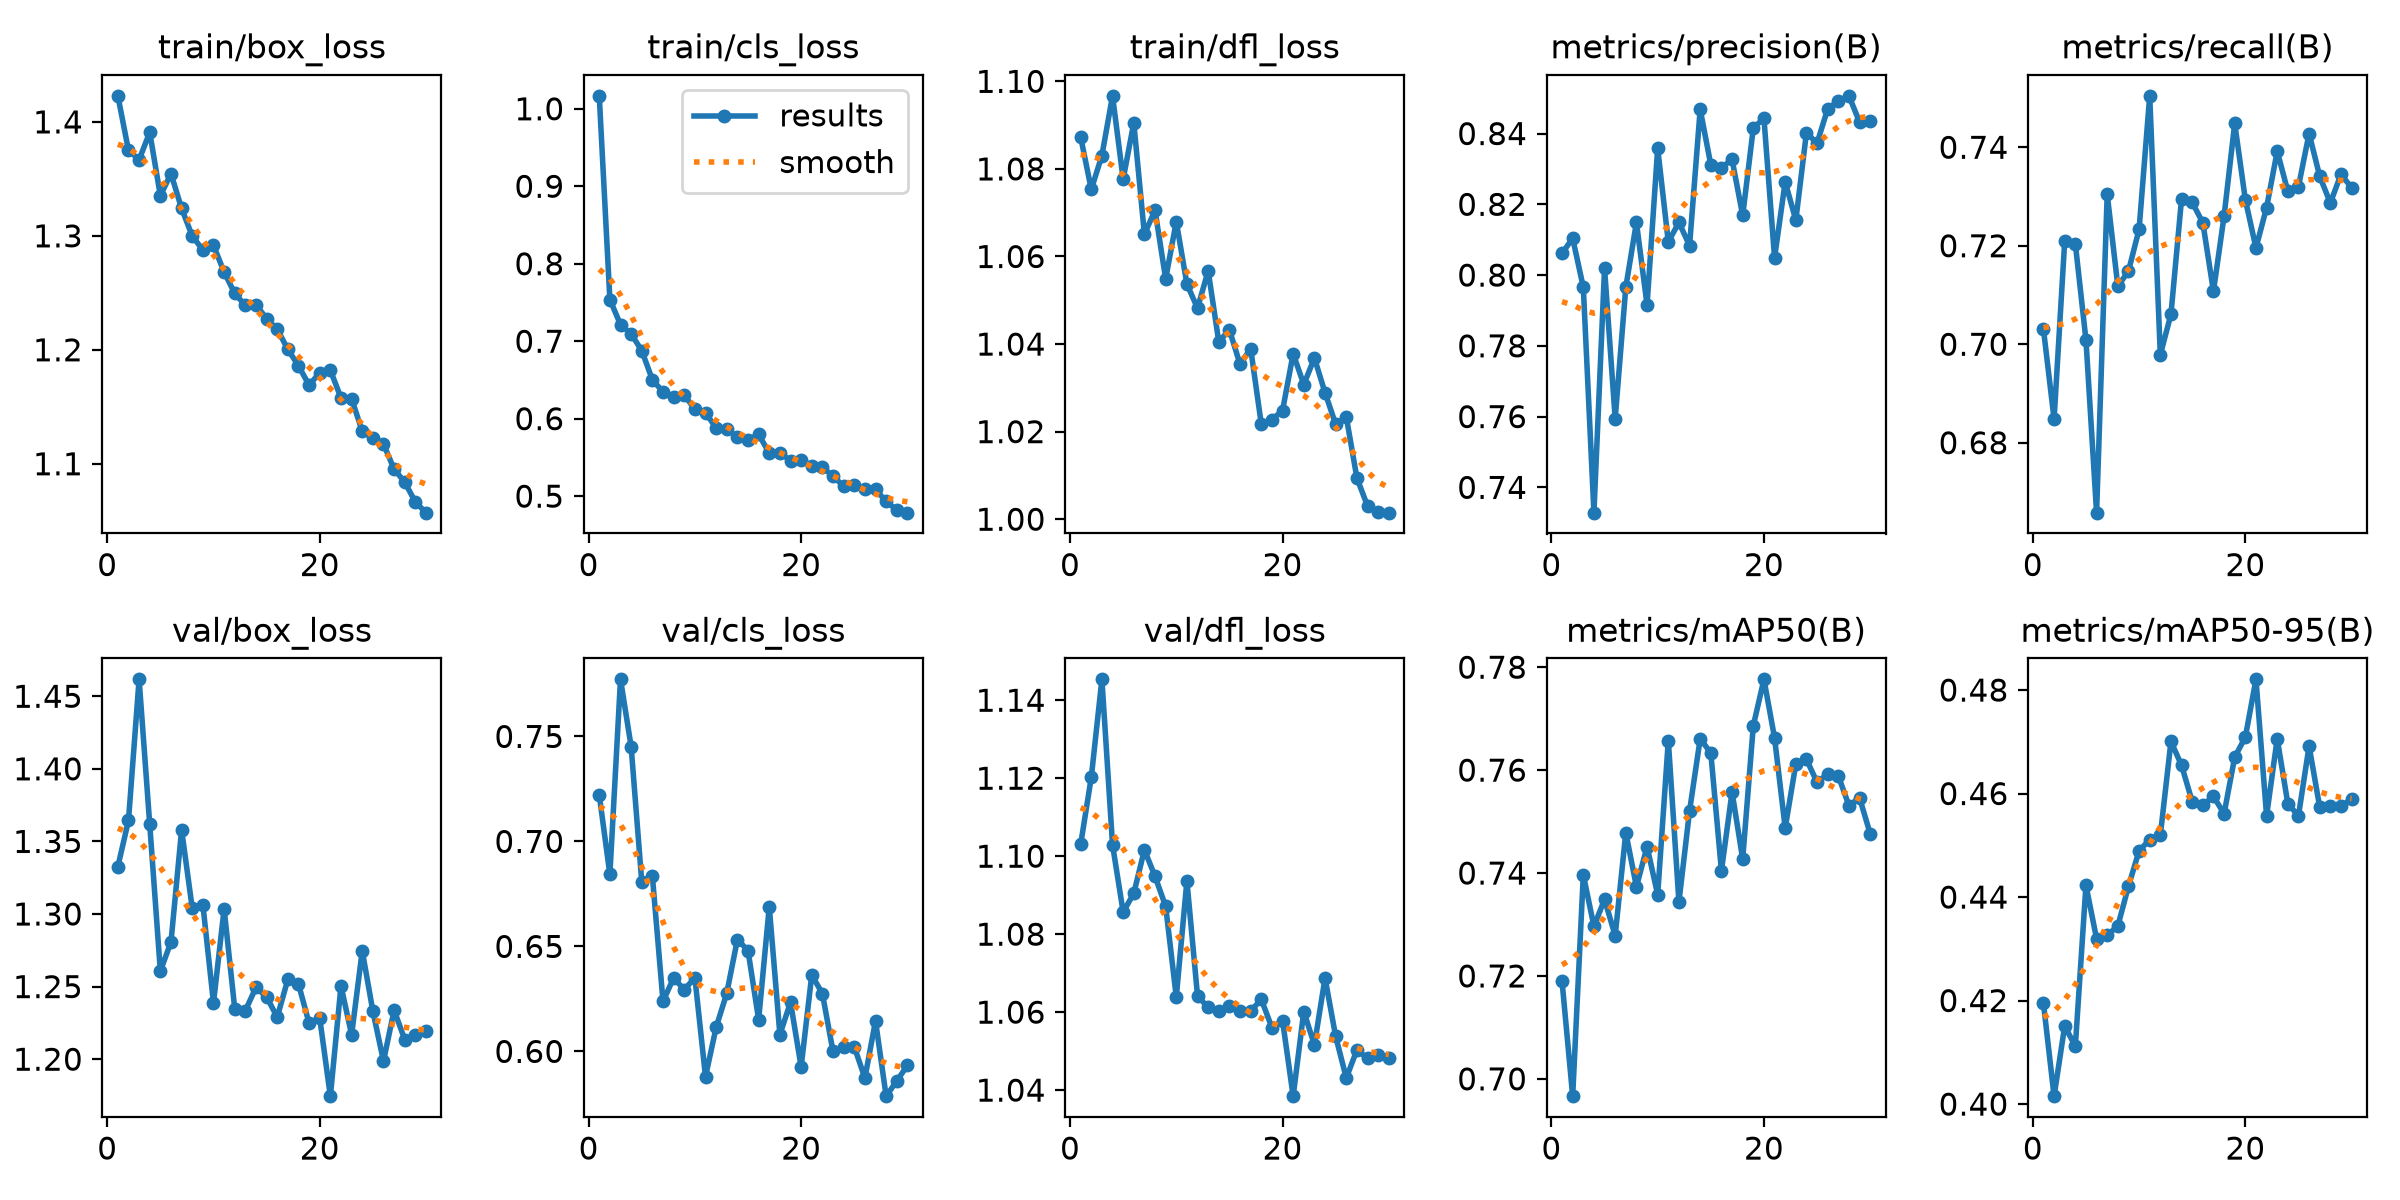
\includegraphics[width=\linewidth,height=0.66\textheight,keepaspectratio]{training_results.png}
\end{column}
\begin{column}{0.29\textwidth}
\small
\textbf{30-epoch recorded run}
\begin{itemize}
  \item Precision: 0.8435
  \item Recall: 0.7318
  \item AP$_{50}$: 0.7476
  \item AP$_{50:95}$: 0.4589
\end{itemize}
\vspace{0.2cm}
\scriptsize These are internal validation logs for the recorded split. They are not presented as final campus-field accuracy.
\end{column}
\end{columns}
\end{frame}

% 12
\begin{frame}{Dashboard and Hardware Prototype}
\begin{columns}[T,onlytextwidth]
\begin{column}{0.65\textwidth}
\phimage{dashboard_live.png}{0.54\textheight}
\centering\scriptsize Live pitch, player labels, ball state, selected-player values, and stream quality.
\end{column}
\begin{column}{0.31\textwidth}
\phimage{hardware_front.jpg}{0.38\textheight}
\vspace{0.15cm}
\scriptsize Light default interface, large primary pitch, responsive player details, text status, no decorative visual effects.
\end{column}
\end{columns}
\vspace{0.12cm}
\scriptsize Build check on August 20: 53 tests and frontend lint/build passed. The relay-only ESP32-S3 firmware compiled at 31\% flash and 8\% dynamic memory.
\end{frame}

% 13
\begin{frame}{Cost and Deployment}
\begin{columns}[T,onlytextwidth]
\begin{column}{0.48\textwidth}
\small
\begin{tabularx}{\linewidth}{X r}
\toprule
\textbf{Budget group} & \textbf{Rs.}\\
\midrule
Five sensor-controller sets & 10,400\\
Battery, regulation, enclosure & 6,000\\
Camera support allowance & 3,000\\
Calibration materials & 1,200\\
\midrule
\textbf{Estimated total} & \textbf{20,600}\\
\bottomrule
\end{tabularx}
\vspace{0.25cm}
\scriptsize The available PC, domain, and VPS add no new cost in this estimate. Invoice values will replace planning values.
\end{column}
\begin{column}{0.49\textwidth}
\centering
\includegraphics[width=\linewidth,height=0.58\textheight,keepaspectratio]{08_deployment.png}
\end{column}
\end{columns}
\end{frame}

% 14
\begin{frame}{Team Contributions and Current Progress}
\begin{columns}[T,onlytextwidth]
\begin{column}{0.51\textwidth}
\scriptsize
\begin{tabularx}{\linewidth}{p{1.6cm}X}
\toprule
\textbf{Member} & \textbf{Primary area}\\
\midrule
Siddartha & Coordination, vision, tactics, integration\\
Raghav & Wearable hardware, firmware, validation\\
Bibek & ML data, fusion models, evaluation\\
Suyogya & Tactical indicators, dashboard UX\\
Om & Acquisition, sync, calibration, tests\\
\bottomrule
\end{tabularx}
\end{column}
\begin{column}{0.46\textwidth}
\textbf{Engineering milestone coverage}\par
\vspace{0.25cm}
\statusbar{O1 Integrated streams}{80}{tietmaroon}\\[0.25cm]
\statusbar{O2 Wearable}{80}{tietmaroon}\\[0.25cm]
\statusbar{O3 ML and tactics}{60}{tietmaroon}\\[0.25cm]
\statusbar{O4 Evaluation}{40}{tietmaroon}
\vspace{0.35cm}
\scriptsize Five defined milestones per objective. Coverage is not an accuracy score.
\end{column}
\end{columns}
\end{frame}

% 15
\begin{frame}{Future Work and Panel Demonstration}
\begin{columns}[T,onlytextwidth]
\begin{column}{0.58\textwidth}
\small
\textbf{Next evidence}
\begin{itemize}
  \item Controlled camera calibration and 20-event sync test
  \item Reference HR, SpO$_2$, IMU, and GPS protocol
  \item Reviewed campus tracks, ball positions, identities, and events
  \item Locked campus detection and tracking evaluation
  \item Later-session workload-model study after the data gate
  \item Coach usability and failure-case review
\end{itemize}
\end{column}
\begin{column}{0.38\textwidth}
\textbf{Panel demo flow}
\begin{enumerate}
  \item Pair and check wearable
  \item Calibrate and start session
  \item Show live tracks and telemetry
  \item Verify one synchronised event
  \item Correct one identity
  \item Explain one tactical/load event
  \item Reconnect local sensor processor
\end{enumerate}
\end{column}
\end{columns}
\vfill
{\Large\bfseries\color{tietmaroon} One timeline. Traceable evidence. Useful coaching decisions.}
\end{frame}

\end{document}
